\section{Diameter information}
\label{compact:diameter}

\paragraph{A prescribed diameter.}
The joint envelope also admits an exact diameter restriction. The
diameter may be an upper bound or a prescribed value; the domain
otherwise varies.

\begin{theorem}[The joint envelope with diameter information]
\label{jointdiam:main}
Assume \eqref{boundarygap:assumptions} and let $D>0$. For $g,P>0$ put
\begin{equation}\label{jointdiam:definition}
 \begin{gathered}
 h=\min\{g,P^2/m,PD\},\qquad
 \rho_-=h^2/P^2,\qquad \rho_+=\min\{h/m,D^2\},\\
 \mathcal J_D(g,P)=\max_{\rho_-\le\rho\le\rho_+}V(h,\rho).
 \end{gathered}
\end{equation}
Set $\mathcal J_D(g,0)=\mathcal J_D(0,P)=0$. Then
\[
 G(x)\le g,\quad \|\nabla f(x)\|\le P,\quad
 \operatorname{diam}Q\le D
 \quad\Longrightarrow\quad
 \delta(x)\le\mathcal J_D(g,P).
\]
The bound is sharp for these three upper bounds. The same supremum
holds with $\operatorname{diam}Q=D$, and is approached by smooth
functions on neighborhoods of triangles with nonempty interior in
$\mathbb R^2$.

For prescribed positive values $G(x)=g$ and $\|\nabla f(x)\|=P$,
the class is nonempty exactly when $g\le PD$. Whenever it is
nonempty, its supremum is again $\mathcal J_D(g,P)$, whether the
diameter is bounded by $D$ or fixed at $D$.
\end{theorem}

For $H_1=0$ put
$\beta=(H_0^2-2mH_0-m^2)/(4H_0)$. Then
\begin{equation}\label{jointdiam:constant}
 \mathcal J_D(g,P)=
 \begin{cases}
 h+\beta\rho_+,&\beta\ge0,\\
 h+\beta\rho_-,&\beta<0.
 \end{cases}
\end{equation}
For example, $m=1$, $H_0=4$, $H_1=0$, $g=1$, $P=2$ and
$D=3/5$ give
\[
 \beta=7/16,\qquad
 \mathcal J_D(1,2)=463/400<23/16=\mathcal J(1,2).
\]
Both observations can be exact, since $g=1<6/5=PD$.
For $H_1>0$ and $\mathcal S(h)\le0$, radius monotonicity gives
\begin{equation}\label{jointdiam:ordinary}
 \mathcal J_D(g,P)=V(h,\rho_-)
       \le h+\rho_-\mathcal S(h)\le h.
\end{equation}
Thus the ordinary-gap regime still needs only one switch equation,
or the displayed algebraic upper bound.

\begin{corollary}[The norm envelope with diameter information]
\label{jointdiam:norm}
For $P>0$ let $r_D=\min\{D,P/m\}$ and $q=\max\{P-mD,0\}$. The
sharp norm-only bound with diameter at most $D$ is
\begin{equation}\label{jointdiam:norm-formula}
 \mathcal E_D(P)=\mathcal J_D(PD,P)
       =A(P,r_D)=\mathcal E_q(P).
\end{equation}
It remains sharp with both $\|\nabla f(x)\|=P$ and
$\operatorname{diam}Q=D$. Set $\mathcal E_D(0)=0$.
If $H_1=0$ and $P\ge mD$, then
\begin{equation}\label{jointdiam:norm-constant}
 \mathcal E_D(P)=PD+\beta D^2.
\end{equation}
For fixed $D$ this is an affine function of $P$.
\end{corollary}

\begin{figure}[htbp]
\centering
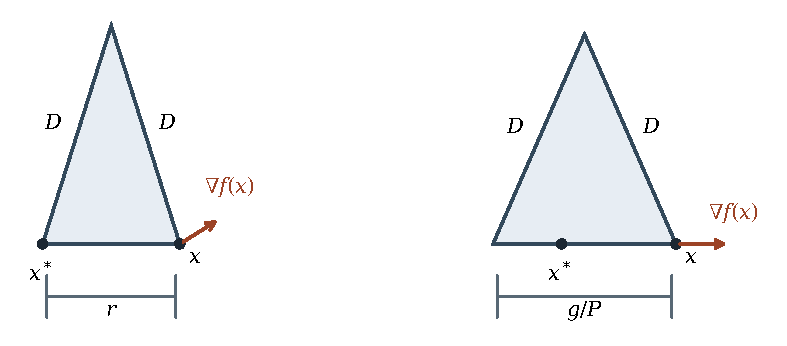
\includegraphics[width=0.9\linewidth]{figures/diameter_geometry.pdf}
\caption{Sharpness constructions for feasible exact observations. Left: gap-active data, $g\le P^2/m$. Right: norm-active data, $P^2/m<g\le PD$. Both sloping sides have length $D$.}
\label{jointdiam:geometry}
\end{figure}

\paragraph{Proof of Theorem~\ref{jointdiam:main}.}
The definitions give $0<\rho_-\le\rho_+$; continuity of $V$ ensures
that the maximum exists. For a nonoptimal source,
write $r=\|x-x^*\|$ and let $p$ be its terminal radial derivative.
Shifted RSI and constrained minimality give
$mr\le p\le P$, while $pr\le G(x)\le g$ and $r\le D$. Hence
\[
 pr\le\min\{g,P^2/m,PD\}=h,\qquad
 r\le R:=\min\{\sqrt{h/m},D\}.
\]
Put $r_0=h/P\le R$. The radial envelope $A(P,r)$ in
\eqref{joint:radial-identity} is strictly increasing in $r$.
For $r\le r_0$ it bounds the loss by
$A(P,r_0)=V(h,r_0^2)$. For $r\ge r_0$, the terminal cap $h/r$
and initial cap $h/r-mr$ bound it by $V(h,r^2)$. This proves
\eqref{jointdiam:definition}. A zero gap or zero norm forces zero
error by shifted RSI. The zero bound is attained at the minimizer
of a quadratic on a triangle of diameter $D$.

For sharpness, choose a maximizing radius $\rho$, and put
\[
 r=\sqrt\rho,\quad p=h/r,\quad q=p-mr,\quad
 c=\sqrt{P^2-p^2},\quad a_D=\sqrt{D^2-r^2/4}.
\]
The scalar construction in Lemma~\ref{compact:radial} gives
smooth functions $u_j$ on neighborhoods of $[0,r]$ with
\[
 \begin{gathered}
 u_j(0)=0,\quad u_j'(0)=q,\quad u_j'(r)=p,\quad
 u_j'(s)-q\ge ms,\\
 |u_j''(s)|\le H_0+H_1u_j(s),\qquad
 u_j(r)\longrightarrow V(h,\rho).
 \end{gathered}
\]
Define
\[
 Q=\operatorname{conv}\{(0,0),(r,0),(r/2,a_D)\},\qquad
 f_j(s,y)=u_j(s)+cy+my^2/2.
\]
The two sloping sides have length $D$ and the base has length
$r\le D$, so $Q$ has diameter exactly $D$ and nonempty interior.
Its points satisfy $0\le s\le r$ and $y\ge0$. The unique minimizer
is $(0,0)$, and throughout $Q$,
\[
 \langle\nabla f_j(s,y)-\nabla f_j(0,0),(s,y)\rangle
       =(u_j'(s)-q)s+my^2\ge m(s^2+y^2),
\]
\[
 \|\nabla^2f_j(s,y)\|
       =\max\{|u_j''(s)|,m\}
       \le H_0+H_1u_j(s)\le H_0+H_1f_j(s,y).
\]
At $(r,0)$ the gradient is $(p,c)$, of norm $P$. Its linear
pairing is minimized at $(0,0)$, so the full gap is $pr=h\le g$.
The source loss tends to $\mathcal J_D(g,P)$. This proves sharpness
for upper bounds, even with diameter fixed exactly.

For exact positive observations, $g\le PD$ is necessary by
$G(x)\le\|\nabla f(x)\|\operatorname{diam}Q$. If also
$g\le P^2/m$, then $h=g$, and the preceding construction already
has both observations exact. If $P^2/m<g\le PD$, set
\[
 r=P/m,\qquad a=g/P-r,\qquad \ell=r+a=g/P\le D.
\]
Use smooth scalar profiles on $[0,r]$ with initial slope zero
and terminal slope $P$, approaching $\mathcal E(P)$. Their
smoothing is confined to the interior switch, so near zero
they agree with
\[
 u_+(s)=
 \begin{cases}
 (H_0/H_1)\{\cosh(\sqrt{H_1}s)-1\},&H_1>0,\\
 H_0s^2/2,&H_1=0.
 \end{cases}
\]
Extend them to $[-a,0]$ by this even function. There
$|u_+''|=H_0+H_1u_+$ and $u_+'(s)s\ge ms^2$.
Denote the extension by $u_j$.
On the triangle
\[
 Q=\operatorname{conv}\left\{(-a,0),(r,0),
       \left((r-a)/2,\sqrt{D^2-\ell^2/4}\right)\right\}
\]
put $f_j(s,y)=u_j(s)+my^2/2$. Again $\operatorname{diam}Q=D$,
the minimizer is $(0,0)$, and shifted RSI and the Hessian bound
hold on all of $Q$. The source gradient is $(P,0)$; the linear
oracle selects $(-a,0)$, giving gap $P\ell=g$. The loss tends
to $\mathcal E(P)=\mathcal J_D(g,P)$. All the functions are
smooth on neighborhoods of their triangles.

Formula \eqref{jointdiam:constant} maximizes the affine radius
profile $h+\beta\rho$. Formula \eqref{jointdiam:ordinary} follows
from Corollary~\ref{gapregime:radius-monotone} at $\rho_-$.
For Corollary~\ref{jointdiam:norm}, the gap bound $PD$ follows
from the norm and diameter bounds. In
$\mathcal J_D(PD,P)$ the radius interval is the singleton
$r_D^2$, and its initial slope is
$P-mr_D=\max\{P-mD,0\}=q$. The radial identity and
Proposition~\ref{joint:fixed-slope} give
\eqref{jointdiam:norm-formula}; the constant-curvature radius
formula gives \eqref{jointdiam:norm-constant}.

\paragraph{The full gap with a known diameter.}
For $D>0$ define
\begin{equation}\label{compact:gap-diameter}
 \mathcal B_D(g)=
 \max_{0\le\rho\le\min\{g/m,D^2\}}V(g,\rho),\qquad
 \mathcal B_D(0)=0.
\end{equation}
If $\operatorname{diam}Q\le D$, then
$\delta(x)\le\mathcal B_D(G(x))\le\mathcal B(G(x))$.
This is the exact supremum for a fixed full gap and a diameter
bound. The function $\mathcal B_D$ is continuous and satisfies
\eqref{boundarygap:growth}.

Indeed, the radial upper bound uses $r\le D$, and the smooth
examples on $[0,r]$ from Lemma~\ref{compact:radial} approach
every value with $r\le D$. The same quadratic functions plus
a linear term as in the proof of Theorem~\ref{boundarygap:main}
give the limit $\rho\downarrow0$.
The substitution $\rho=z\min\{g/m,D^2\}$, $z\in[0,1]$, proves
continuity; adding a linear term proves growth without changing
the interval length.

For $H_1=0$,
\[
 \mathcal B_D(g)=g+\max\{0,\beta\}\min\{g/m,D^2\}.
\]
For $H_1>0$, $g>0$, the exact criterion is
\[
 \mathcal B_D(g)=g\quad\Longleftrightarrow\quad\mathcal S(g)\le0.
\]
In the nonpositive case, use
$g\le\mathcal B_D(g)\le\mathcal B(g)=g$.
In the positive case, the first variation
\eqref{gapregime:variation} exceeds $g$ at arbitrarily small
positive radii, which also satisfy $\rho\le D^2$.
For scalar evaluation, apply Proposition~\ref{boundarygap:budget}
on the shorter interval with $\ell=g$.
